\documentclass[11pt, a4paper]{article}
\usepackage{Sweave}
\usepackage{graphicx, verbatim}
\usepackage[utf8]{inputenc}
\usepackage{cite}
\usepackage{authblk}

\begin{document}
\Sconcordance{concordance:roapkg.tex:roapkg.Rnw:%
1 52 1 1 6 2 0 1 1 1 3 1 0 4 1 1 3 1 0 5 1 1 3 1 0 2 %
1 3 0 1 2 1 1 1 2 1 0 1 1 3 0 1 2 1 3 87 0 2 2 4 0 2 %
2 4 0 2 2 4 0 1 2 2 1 1 2 5 0 1 2 3 1 1 2 18 0 1 2 6 %
1 1 2 18 0 2 2 4 0 1 2 3 1 1 2 1 0 2 1 30 0 1 1 31 0 %
1 2 5 1 1 3 2 0 1 3 1 0 5 1 1 3 1 0 3 1 1 2 1 0 1 1 1 %
3 1 0 1 1 1 2 1 0 1 3 1 0 2 1 3 0 1 2 1 1 1 3 5 0 2 2 %
1 0 1 1 30 0 1 1 31 0 2 2 4 0 2 2 4 0 1 2 2 1}

\title{Univariate and Multivariate Outlier Analysis for Genomic Data: The \textbf{roa} package}
\author[1,2]{Kylie Ainslie}
\author[1,2]{Jeanne Kowalski} 
  \affil[1]{Department of Biostatistics and Bioinformatics, Rollins School of Public Health, Emory University, Atlanta, GA}
  \affil[2]{Biostatistics and Bioinformatics Shared Resource, Winship Cancer Institute, Emory University, Atlanta, GA}


%\SweaveOpts{concordance=TRUE}
\maketitle


\section{Introduction}
The cancer genome is exceedingly complex due to the high amount of genetic instability. Differential gene expression methodologies have long been employed to identify the unstable genes that lead to tumor initiation and progression. In some cancers, such as multiple myeloma (MM), genetic instability is seen mainly as translocations that result in abnormal gene expression. However, many of these instability events occur in only a subset of patients, making detection via traditional differential gene expression methods difficult. A classic example of such a disruption is the FGFR3-IGH translocation in MM, which occurs in only 15-20\% of patients \cite{bergsagel, segges}. Patients with the FGFR3-IGH, t(4;14) translocation have abnormally high expression of FGFR3 \cite{bergsagel, chesi}, and have been associated with poorer prognosis \cite{segges}. Thus, instability events in a fraction of patients are of interest, but are difficult to detect. 

Several outlier detection methods have been developed to detect gene expression outliers, such as FGFR3. These outlier methods have succeeded in identifying unstable genes. Tomlins et al. identified the TMPRSS2-ETS fusion in prostate cancer using the Cancer Profile Outlier Analysis (COPA) \cite{copa}. Other previously developed outlier methods include the Outlier Sum Statistic (OSS) \cite{oss} and Gene Tissue Index (GTI) \cite{gti}. While these three statistics perform similarly, they differ drastically in the genes they rank the highest \cite{gti}. This package provides two integrated outlier analysis approaches. The first, a univariate approach, calculates each outlier statistic separately in addition to the variance and then applies a change point model \cite{cpm} to identify outlier genes based on each statistic. The separate gene lists can then be further filtered by instersection. The second approach, a multivariate approach, combines the three outlier statistics into a score statistic and then identifies outlier genes using a change point model \cite{cpm}.

The purpose of this paper is to describe the \textbf{roa} package which provides both univariate and multivariate approaches to outlier identification. Many previosly developed outlier methods and packages are designed for gene expression microarray data \cite{gti,oss,copa,multi,zodet}. Unlike existing R packages, the \textbf{roa} package can be used with numerous types of biological data in addition to gene expression microarray data, such as RNA-Seq, methylation, and copy number data. The \textbf{roa} package also allows the use of a multivariate approach to identify outliers.

Section 2 of this paper provides some background into the methods used within this package. Section 2.1 describes the previously developed outlier methods used in this package. Section 3 provides an overview of the univariate approach along with examples of usage. Section 4 provides an overview of the multivariate approach and examples of usage. In Section 5, additional capabilities of \textbf{roa} are discussed.

\section{Background}
The previously developed outlier statistics (COPA, OSS, and GTI) were designed to find outliers in a two group context (disease samples relative to normal samples) \cite{gti,oss,copa}. In practice it is not always possible to have both disease and normal samples. This package features these three statistics in both their two group context (uv.outlier2 and mv.outlier2) and in their single group (disease only samples) context (uv.outlier and mv.outlier).

\subsection{Existing Methods}
The COPA statistic and OSS were developed based on the t-statistic replacing the mean and standard deviation with the median and median absolute deviation, respectively \cite{gti,oss,copa}. Borrowing notation from Mpindi et al. 2011, the COPA statistic is defined as
\begin{equation}
COPA_j=q_r(\tilde{x}_{ij})=\frac{q_r(x_{ij}:i \in C_2)-med_j}{mad_j},
\end{equation}
where $ q_r(x_{ij}:i \in C_2) $ is the rth percentile (in this paper we use r=85) of disease samples’ standardized gene expression, $x_{ij}$ is the gene expression of sample i for gene j, $med_j$ is the median expression value among all samples for gene j, and $mad_j$ is the median absolute deviation of all samples for gene j (6).  
	The OS statistic is defined as
\begin{equation}
OSS_j=\frac{\sum_{i\in O_j}(x_{ij}-med_j)}{mad_j},
\end{equation},
where $O_j$ is the set of outlier samples \\
$(O_j={i: x_{ij} > q_{75}(x_{mj}:m=1,…n)+IQR(x_{mj}:m=1,\dots n)})$, $x_{ij}$ is the gene expression of sample i for gene j, medj is the median expression value among all samples for gene j, and $mad_j$ is the median absolute deviation of all samples for gene j \cite{gti,oss}. 
The GTI was adapted from economics to weight an outlier’s outlying-ness. The GTI statistic is defined as
\begin{equation}
GTI_j=\frac{T_j}{n_j}\times \frac{(A_j-B_j)}{A_j},
\end{equation}
where $T_j$ is the number of samples with expression values about the cut-off for gene j, $n_j$ is the total number of samples for gene j, $A_j$ is the average expression of samples above the cut-off for gene j, and $B_j$ is the cut-off value for gene j \cite{gti}. We used the standard cut-off $q_{75}$ + IQR.

\section{Univariate Outlier Analysis}
\subsection{Data}
For the purposes of this vignette, the following code will be used to simulate microarray gene expression data. For use with \textbf{roa} data should be formatted with samples down the rows and genomic IDs across the columns. Row names should be the sample IDs and column names should be the genomic IDs. Some genomic IDs, such as microarray gene expression probes, begin with numbers. R does not allow column names to start with a number, so an "X" is added to the ID. To make sure IDs can be appropriately matched back to any annotation files, all functions in \textbf{roa} have an logical option, num.id, to indicate whether the IDs being with a number. 
\begin{Schunk}
\begin{Sinput}
> #generate non-outlier data
>  set.seed(0)
>  sim.data<-matrix(c(rnorm(1000*200,0,1)),nrow=200)
> #generate outlier gene expression
>   y<-matrix(rnorm(200*10,0,1),nrow=200)
>   m<-max(sim.data,y)
>   c<-c(rep(m,20),rep(0,180))
>   test.genes<-y+c
>   data<-cbind(test.genes,sim.data)
> #add column names
>   pre<-"test"
>   suf<-seq(1:10)
>   prefix<-"gene"
>   suffix<-seq(1:1000)
>   colnames(data)<-c(paste(pre,suf,sep=""),paste(prefix,suffix,sep=""))
>   rownames(data)<-c(paste("sample",seq(1:200),sep=""))
> #create annotation file
>   p<-"gene.symbol"
>   s<-seq(1:1010)
>   annot<-data.frame(ID=colnames(data),Gene=paste(p,s,sep=""))
\end{Sinput}
\end{Schunk}
\subsection{Univariate Approach}
The univariate approach incorporates all three previously mentioned outlier methods in addition to a simple variance estimate to identify a robust list of outliers. Each outlier statistic is calculated for each gene then, using either a change point model (using the \textbf{cpm} R package \cite{cpm}) or a user-defined cut-off, outliers are determined for each statistic. To apply the univariate approach to a dataset use the uv.outlier (for data containing only disease samples) or uv.outlier2 function (for data containing both disease and normal samples). Detailed usage of the single group functionality of \textbf{roa} follows. For detailed examples of how to use the two group functions available in \textbf{roa} see Section 6.
\begin{Schunk}
\begin{Sinput}
> library(roa)
> uv.outlier(data,num.id=F)
\end{Sinput}
\end{Schunk}
If an annotation file is not specified four method-specific lists of outliers are outputted. If an annotation file is specified, a single list of outliers is outputted with a column that indicates the method that selected each outlier. The lists of outlier genes from each of the statistics can be further filtered by intersection to identify genes in common among all four or three of the four method-specific lists.
\begin{Schunk}
\begin{Sinput}
> uv.outlier(data,annotation=annot,annID=1,annName=2,common.genes=T,
+            num.id=F)
\end{Sinput}
\begin{Soutput}
$Outliers
        ID           Gene      Value Stat
1    test1   gene.symbol1  0.1783530  GTI
2    test2   gene.symbol2  0.1547711  GTI
3    test3   gene.symbol3  0.1541250  GTI
4    test4   gene.symbol4  0.1585624  GTI
5    test5   gene.symbol5  0.1512725  GTI
6    test6   gene.symbol6  0.1353544  GTI
7    test7   gene.symbol7  0.1611340  GTI
8    test8   gene.symbol8  0.1705163  GTI
9    test9   gene.symbol9  0.1562230  GTI
10  test10  gene.symbol10  0.1631958  GTI
11  gene88  gene.symbol98  0.1050203  GTI
12 gene321 gene.symbol331  0.1192038  GTI
13 gene326 gene.symbol336  0.1193138  GTI
14 gene423 gene.symbol433  0.1087650  GTI
15 gene576 gene.symbol586  0.1111786  GTI
16 gene713 gene.symbol723  0.1498315  GTI
17 gene776 gene.symbol786  0.1291890  GTI
18 gene939 gene.symbol949  0.1091213  GTI
19 gene945 gene.symbol955  0.1158901  GTI
20   test3   gene.symbol3  1.3392260 COPA
21   test5   gene.symbol5  1.5537824 COPA
22   test9   gene.symbol9  1.3891657 COPA
23 gene423 gene.symbol433  1.3188595 COPA
24 gene467 gene.symbol477  1.3049081 COPA
25 gene513 gene.symbol523  1.3829467 COPA
26 gene568 gene.symbol578  1.3678889 COPA
27 gene606 gene.symbol616  1.3592691 COPA
28 gene614 gene.symbol624  1.3222921 COPA
29 gene711 gene.symbol721  1.3229690 COPA
30 gene713 gene.symbol723  1.3286257 COPA
31 gene842 gene.symbol852  1.3278992 COPA
32 gene982 gene.symbol992  1.3560150 COPA
33   test1   gene.symbol1 87.7868650  OSS
34   test2   gene.symbol2 74.4776175  OSS
35   test3   gene.symbol3 64.2546999  OSS
36   test4   gene.symbol4 80.4086621  OSS
37   test5   gene.symbol5 80.5912136  OSS
38   test6   gene.symbol6 55.6073216  OSS
39   test7   gene.symbol7 64.9406565  OSS
40   test8   gene.symbol8 69.5377068  OSS
41   test9   gene.symbol9 83.5613825  OSS
42  test10  gene.symbol10 64.9254744  OSS
43  gene88  gene.symbol98 30.1306480  OSS
44 gene321 gene.symbol331 33.0971273  OSS
45 gene326 gene.symbol336 30.8513613  OSS
46 gene423 gene.symbol433 32.2585381  OSS
47 gene713 gene.symbol723 39.8336533  OSS
48 gene776 gene.symbol786 31.2638678  OSS
49 gene945 gene.symbol955 32.7184197  OSS
50   test1   gene.symbol1  2.8101980  Var
51   test2   gene.symbol2  2.8216016  Var
52   test3   gene.symbol3  2.7904783  Var
53   test4   gene.symbol4  2.7417140  Var
54   test5   gene.symbol5  2.9983425  Var
55   test6   gene.symbol6  2.8762020  Var
56   test7   gene.symbol7  2.5463137  Var
57   test8   gene.symbol8  2.9604481  Var
58   test9   gene.symbol9  2.7600413  Var
59  test10  gene.symbol10  2.6867408  Var
60 gene599 gene.symbol609  1.3145743  Var

$Common_Genes
         ID           Gene Methods
3     test3   gene.symbol3       4
5     test5   gene.symbol5       4
9     test9   gene.symbol9       4
1     test1   gene.symbol1       3
2     test2   gene.symbol2       3
31    test3   gene.symbol3       3
4     test4   gene.symbol4       3
51    test5   gene.symbol5       3
6     test6   gene.symbol6       3
7     test7   gene.symbol7       3
8     test8   gene.symbol8       3
91    test9   gene.symbol9       3
10   test10  gene.symbol10       3
433 gene423 gene.symbol433       3
723 gene713 gene.symbol723       3
\end{Soutput}
\end{Schunk}
The default method of identifying a threshold by which outliers are identified is using the Mann-Whitney statistic in a nonparametric change point model framework. The \textbf{cpm} package is used to identify the change point and can be implemented using the Student-t, Bartlett, and GLR statistics for sequences known to be Gaussian; Fisher's Exact Test statistic for Bernoulli sequences; Exponential statistic for Exponential sequences, and Mann-Whitney, Mood, Lepage, Kolmogorov-Smirnov, and Cramer-von-Mises statistics for sequences in which the distribution is not known \cite{cpm}. For more information on \textbf{cpm}, see the \textbf{cpm} manual available at <http://www.gordonjross.co.uk/cpm.pdf>.
\begin{Schunk}
\begin{Sinput}
> uv.outlier(data,cpmtype="Mann-Whitney",num.id=F)
\end{Sinput}
\end{Schunk}
In addition to the identification of an outlier threshold using a change point model framework, a user-defined cut-off can be specified.
\begin{Schunk}
\begin{Sinput}
> uv.outlier(data,p=0.95,num.id=F)
\end{Sinput}
\end{Schunk}
COPA, OSS, and GTI were developed to identify over expressed gene expression outliers. However, all of these statistics have been adapted to identify low-valued outliers, such as under expressed or hypo methylated genes. Specifying under=T in any of the functions will results in the identification of low-valued outliers.   
\begin{Schunk}
\begin{Sinput}
> uv.outlier(data,cut=0.15,under=T,num.id=F)
\end{Sinput}
\end{Schunk}
A results file and threshold figure generated from each list of outliers can be outputted if a path is specified.
\subsubsection{Figures}
In addition to the lists of outliers selected by each outlier statistic, uv.outlier produces a threshold plot for each statistic. If no path indicating where output should be saved is identified, threshold plots are outputted directly into R as one figure. 
\begin{Schunk}
\begin{Sinput}
> uv.outlier(data,num.id=F)
\end{Sinput}
\end{Schunk}
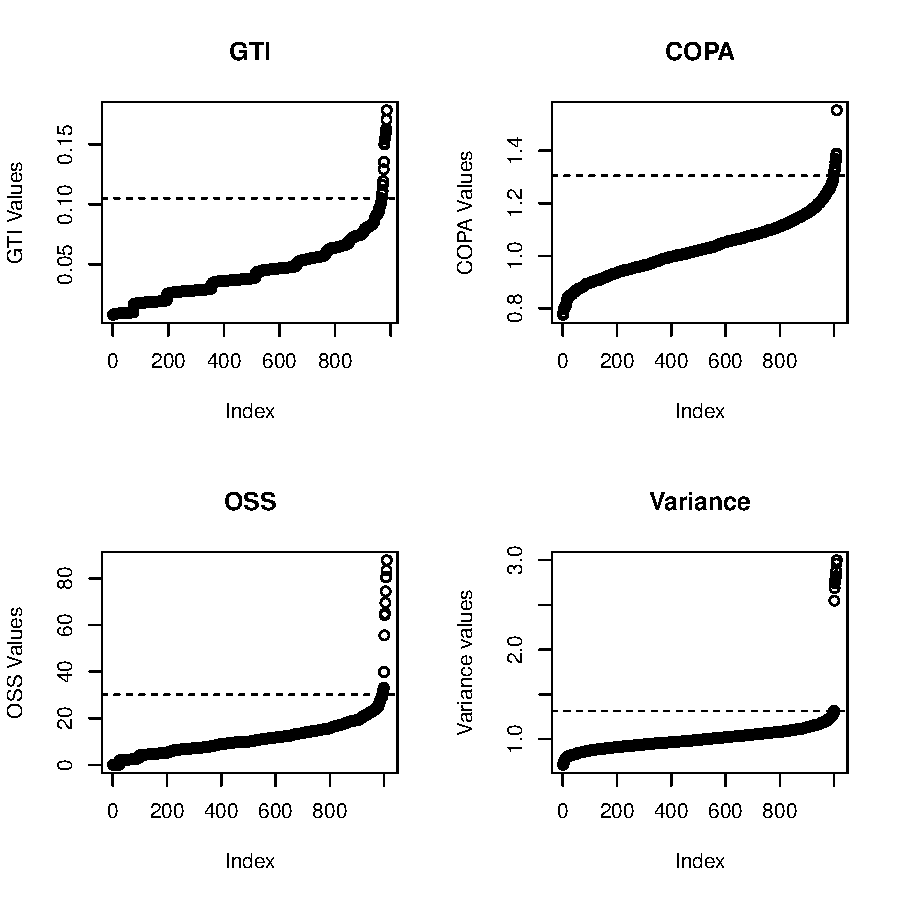
\includegraphics{roapkg-008}
If a path is identified, a jpeg file of the threshold plot and a plot of the D statistics from the change point model \cite{cpm} is output for each outlier statistic.

\subsection{Individual Outlier Statistics}
In addition, if the user would rather identify outliers using only one method instead of all four, each outlier detection method has both a single group and two group function. For example, if an investigator's favorite outlier detection method was the OSS, outliers could be identified using just the OSS. Each individual outlier statistic function can produce a threshold plot showing the threshold by which outlier were identified.
\begin{Schunk}
\begin{Sinput}
> oss(data,num.id=F)
\end{Sinput}
\begin{Soutput}
      gso    Value Stat
1   test1 87.78687  OSS
2   test2 74.47762  OSS
3   test3 64.25470  OSS
4   test4 80.40866  OSS
5   test5 80.59121  OSS
6   test6 55.60732  OSS
7   test7 64.94066  OSS
8   test8 69.53771  OSS
9   test9 83.56138  OSS
10 test10 64.92547  OSS
\end{Soutput}
\end{Schunk}
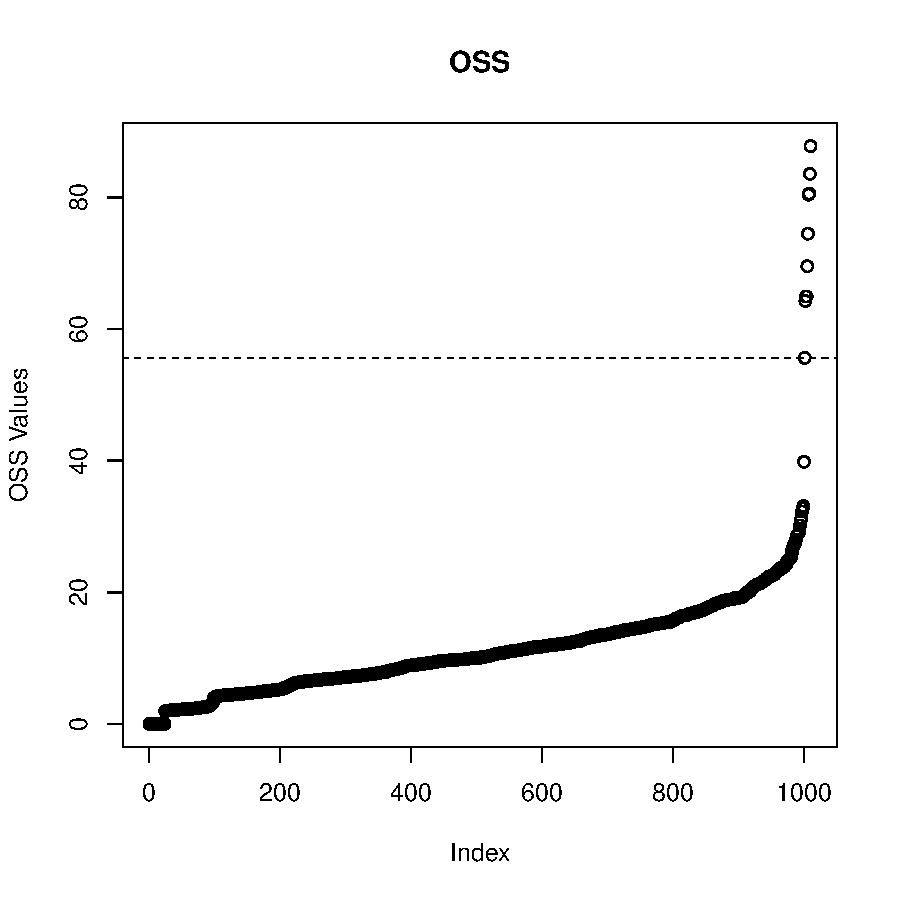
\includegraphics{roapkg-009}

\section{Multivariate Outlier Analysis}
The multivariate approach integrates the COPA, OSS, and GTI statistics into a score statistic to identify outliers. First, each outlier statistic is calculated for each gene. Second, a score statistic is calculated from the three statistics using an identity matrix as the variance-covariance matrix. Let $\mathbf{\theta}_j=(c_j,o_j,g_j)^T$ be the vector of outlier statistics calculated for gene $j$, $j=1,2,\dots,n$. Let $\mathbf{V}=\mathbf{I}_3$ be the variance-covariance matrix. The score statistic for gene $j$ is thus,
\begin{equation}
S_j=\mathbf{\theta}_j^T \mathbf{V} \mathbf{\theta}_j.
\end{equation}
Finally, outliers are determined by applying either a change point model \cite{cpm} or a user-defined cut-off to the vector of score statistics, $\mathbf{S}=(S_1,S_2,\dots,S_n)^T$. The threshold by which outliers are identified can be visualized by the outputted threshold plot. Similarly to the univariate approach, the multivariate approach can be used with single group data (mv.outlier) or two group data (mv.outlier2).
\begin{Schunk}
\begin{Sinput}
> mv.outlier(data,num.id=F)
\end{Sinput}
\begin{Soutput}
       ID   Gene    Score
1   test1  test1 7707.889
2   test2  test2 5548.106
3   test3  test3 4130.484
4   test4  test4 6466.375
5   test5  test5 6497.381
6   test6  test6 3093.425
7   test7  test7 4218.694
8   test8  test8 4836.479
9   test9  test9 6984.459
10 test10 test10 4216.749
\end{Soutput}
\end{Schunk}
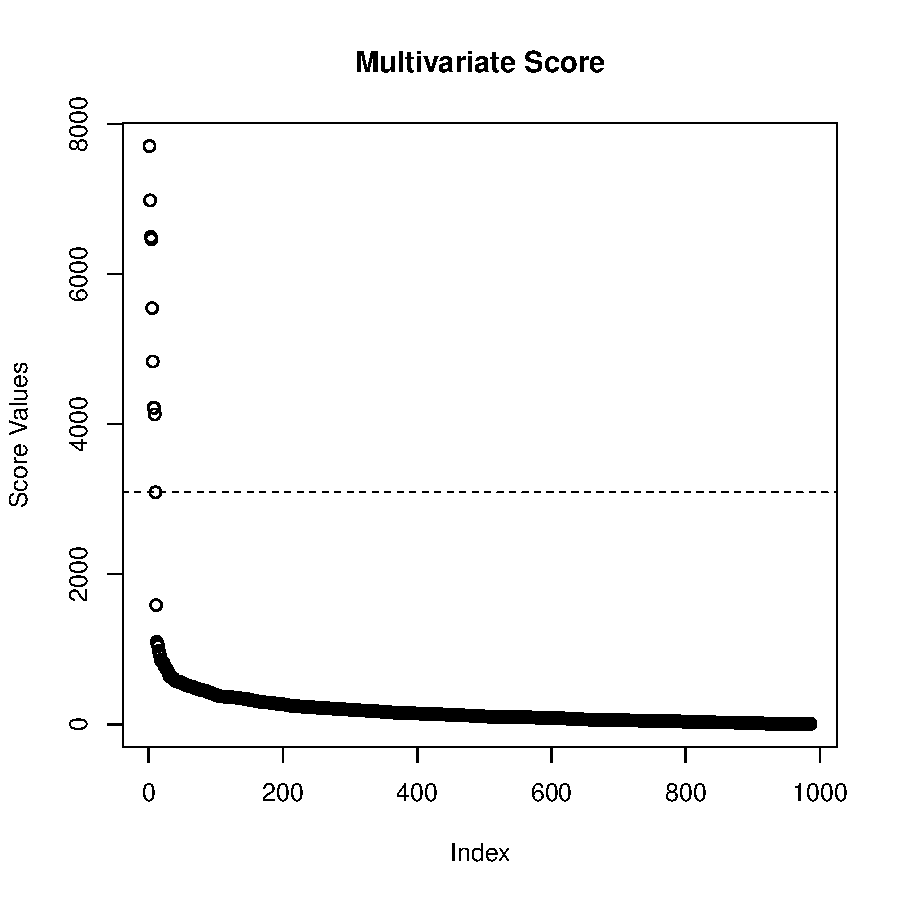
\includegraphics{roapkg-010}
As with the univariate approach, the default method of identifying an outlier threshold is using a change point model framework with the Mann-Whitney statistic. As mentioned in Section 3.1, other parametric and nonparametric statistics can be implemented with the change point model framework \cite{cpm}. A user-defined cut-off can also be specified for outlier identification.
\begin{Schunk}
\begin{Sinput}
> mv.outlier(data,p=0.95,num.id=F)
\end{Sinput}
\end{Schunk}
\section{Additional Capabilities}
\subsection{Outlying Samples}
Often when an outlier is identified it is of interest to determine which samples had outlying values,i.e., which samples caused that outlier to be an outlier. If those samples have a common trait, it may be indicative of a subgroup within the samples. The function outlying.samples provides the ability to determine which samples have outlying values. When using outlying.samples, a list with two components is returned. The first component is a matrix with each row representing a sample and each column representing an outlier. A 1 in element [i,j] indicates that sample i has an outlying value for outlier j. The second component is a two column matrix with the sample IDs in column one and an indicator of whether each sample has an outlying value in at least one outlier.

\begin{Schunk}
\begin{Sinput}
> out<-mv.outlier(data,num.id=F)
> os<-outlying.samples(data,outliers=out[,1])
> os$by.outlier[1:25,1:8]
\end{Sinput}
\begin{Soutput}
         ID test1 test2 test3 test4 test5 test6 test7
1   sample1     1     1     1     1     1     1     1
2   sample2     1     1     1     1     1     1     1
3   sample3     1     1     1     1     1     1     1
4   sample4     1     1     1     1     1     1     1
5   sample5     1     1     1     1     1     1     1
6   sample6     1     1     1     1     1     1     1
7   sample7     1     1     1     1     1     1     1
8   sample8     1     1     1     1     1     1     1
9   sample9     1     1     1     1     1     1     1
10 sample10     1     1     1     1     1     1     1
11 sample11     1     1     1     1     1     1     1
12 sample12     1     1     1     1     1     1     1
13 sample13     1     1     1     1     1     1     1
14 sample14     1     1     1     1     1     1     1
15 sample15     1     1     1     1     1     1     1
16 sample16     1     1     1     1     1     1     1
17 sample17     1     1     1     1     1     1     1
18 sample18     1     1     1     1     1     1     1
19 sample19     1     1     1     1     1     1     1
20 sample20     1     1     1     1     1     1     1
21 sample21     0     0     0     0     0     0     0
22 sample22     0     0     0     0     0     0     0
23 sample23     0     0     0     0     0     0     0
24 sample24     0     0     0     0     0     0     0
25 sample25     0     0     0     0     0     0     0
\end{Soutput}
\begin{Sinput}
> os$sample.ind[1:25,]
\end{Sinput}
\begin{Soutput}
         ID Outlying
1   sample1        1
2   sample2        1
3   sample3        1
4   sample4        1
5   sample5        1
6   sample6        1
7   sample7        1
8   sample8        1
9   sample9        1
10 sample10        1
11 sample11        1
12 sample12        1
13 sample13        1
14 sample14        1
15 sample15        1
16 sample16        1
17 sample17        1
18 sample18        1
19 sample19        1
20 sample20        1
21 sample21        0
22 sample22        0
23 sample23        0
24 sample24        0
25 sample25        0
\end{Soutput}
\end{Schunk}
Note: the full output is not shown above. 
\section{Appendix}
\subsection{Examples using two group functions}
\subsubsection{Data}
The two group functions which allow for the analysis of data that contains normal and disease samples result in the same output as their single group counterparts. The main difference when using the two group functions is the need to specify three different datasets instead of one. The subset of disease samples, the subset of normal samples, and the entire dataset should be specified as data\_ d, data\_ n, and data\_ all, respectively.

\begin{Schunk}
\begin{Sinput}
> #generate normal data
>  norm.data<-matrix(c(rnorm(1010*100,0,1)),nrow=100)
> #generate disease data with 10 outlier genes
>   mydata<-matrix(rnorm(1000*100,0,1),nrow=100)
>   y<-matrix(rnorm(100*10,0,1),nrow=100)
>   m<-max(mydata,y)
>   c<-c(rep(m,20),rep(0,80))
>   test.genes<-y+c
>   dis.data<-cbind(test.genes,mydata)
> #add column names
>   pre<-"test"
>   suf<-seq(1:10)
>   prefix<-"gene"
>   suffix<-seq(1:1000)
>   colnames(dis.data)<-c(paste(pre,suf,sep=""),
+                         paste(prefix,suffix,sep=""))
>   rownames(dis.data)<-c(paste("dis.sample",seq(1:100),sep=""))
>   colnames(norm.data)<-c(paste(pre,suf,sep=""),
+                          paste(prefix,suffix,sep=""))
>   rownames(norm.data)<-c(paste("norm.sample",seq(1:100),sep=""))
> #complete data
>   all.data<-rbind(dis.data,norm.data)
> #create annotation file
>   p<-"gene.symbol"
>   s<-seq(1:1010)
>   annot<-data.frame(ID=colnames(dis.data),Gene=paste(p,s,sep=""))
\end{Sinput}
\end{Schunk}
\subsubsection{Examples}
Below is an example of using the two group multivariate function.
\begin{Schunk}
\begin{Sinput}
> example<-mv.outlier2(dis.data,norm.data,all.data,annotation=annot,
+               annID=1,annName=2,num.id=FALSE)
\end{Sinput}
\end{Schunk}
Suppose we want to identify the outlying samples. The two-group outlier statistics are calculated to identify outliers in the disease group relative to the normal group, so we only need to specify the disease dataset to find outlying samples. Note, the output shown below has been shortened and only shows the first 25 samples.
\begin{Schunk}
\begin{Sinput}
> os2<-outlying.samples(dis.data,outliers=example[,1])
> os2$by.outlier[1:25,1:8]
\end{Sinput}
\begin{Soutput}
             ID test2 test3 test4 test5 test6 test7 test8
1   dis.sample1     1     1     1     1     1     1     1
2   dis.sample2     0     1     1     1     1     1     1
3   dis.sample3     1     0     1     1     0     0     1
4   dis.sample4     1     1     0     1     1     0     0
5   dis.sample5     0     1     1     1     0     0     1
6   dis.sample6     1     0     0     0     1     1     0
7   dis.sample7     0     0     0     1     1     1     1
8   dis.sample8     1     1     1     1     1     1     1
9   dis.sample9     1     1     0     1     1     1     1
10 dis.sample10     1     1     1     0     1     1     1
11 dis.sample11     1     1     1     0     1     1     1
12 dis.sample12     1     1     1     1     1     1     1
13 dis.sample13     0     1     1     1     0     1     1
14 dis.sample14     1     1     1     0     1     1     0
15 dis.sample15     1     1     0     0     1     1     1
16 dis.sample16     0     0     1     1     1     1     1
17 dis.sample17     1     0     1     1     0     0     1
18 dis.sample18     1     1     1     1     1     1     1
19 dis.sample19     1     1     1     1     1     0     0
20 dis.sample20     1     1     1     1     0     1     0
21 dis.sample21     0     0     0     0     0     0     0
22 dis.sample22     0     0     0     0     0     0     0
23 dis.sample23     0     0     0     0     0     0     0
24 dis.sample24     0     0     0     0     0     0     0
25 dis.sample25     0     0     0     0     0     0     0
\end{Soutput}
\begin{Sinput}
> os2$sample.ind[1:25,]
\end{Sinput}
\begin{Soutput}
             ID Outlying
1   dis.sample1        1
2   dis.sample2        1
3   dis.sample3        1
4   dis.sample4        1
5   dis.sample5        1
6   dis.sample6        1
7   dis.sample7        1
8   dis.sample8        1
9   dis.sample9        1
10 dis.sample10        1
11 dis.sample11        1
12 dis.sample12        1
13 dis.sample13        1
14 dis.sample14        1
15 dis.sample15        1
16 dis.sample16        1
17 dis.sample17        1
18 dis.sample18        1
19 dis.sample19        1
20 dis.sample20        1
21 dis.sample21        1
22 dis.sample22        0
23 dis.sample23        0
24 dis.sample24        0
25 dis.sample25        0
\end{Soutput}
\end{Schunk}
The two group versions of the univariate outlier analysis and the individual outlier statistic functions have the same arguments as the two group multivariate function.
\begin{Schunk}
\begin{Sinput}
> uv.outlier2(dis.data,norm.data,all.data,num.id=FALSE)
\end{Sinput}
\end{Schunk}
For any function, single group or two group, a user-defined threshold can be identified.
\begin{Schunk}
\begin{Sinput}
> copa2(dis.data,norm.data,all.data,num.id=FALSE,p=0.85)
\end{Sinput}
\end{Schunk}
\bibliography{roa}{}
\bibliographystyle{plain}
\end{document}
